\documentclass[11pt,a4paper]{article}
\usepackage[margin=2.3cm]{geometry}
\usepackage[T1]{fontenc}
\usepackage{lmodern}
\usepackage{amsmath,amssymb}
\usepackage{booktabs,longtable,array}
\usepackage{graphicx}
\usepackage{listings}
\usepackage{xcolor}
\usepackage[hidelinks]{hyperref}
\usepackage{url}
\urlstyle{tt}
\def\UrlBreaks{\do\/\do\_\do\=\do\(\do\)\do\*\do\,\do\.\do\-\do\:\do\+\do\|}

\newcommand{\code}[1]{{\small\path{#1}}}
\newcommand{\qalf}{Q_{\alpha}}
\newcommand{\qbet}{Q_{\beta}}
\newcommand{\qgam}{Q_{\gamma}}
\newcommand{\wrk}{w}
\newcommand{\qmin}{Q_{\alpha,\min}}
\newcommand{\qmax}{Q_{\alpha,\max}}
\newcommand{\note}[1]{\par\smallskip\noindent\fbox{\parbox{0.94\linewidth}{\small #1}}\smallskip}

\lstset{basicstyle=\ttfamily\footnotesize,breaklines=true,columns=fullflexible,
        frame=single,backgroundcolor=\color{black!3},keepspaces=true}

\title{Magnetic contact area $P_{bs}$ and the angles $Q_\alpha$, $Q_\beta$, $Q_\gamma$\\
       of unstructured B2.5 wall faces:\\
       use in the code, boundary conditions, and the geometry prep step}
\author{Technical notes}
\date{\today}

\begin{document}
\maketitle
\tableofcontents

%======================================================================================
\section{Summary}
\begin{itemize}
\item \code{fcPbs} ($P_{bs}$) is the \emph{magnetic contact area} of a face: the face area $S$ times the fraction of
      the field direction that crosses it. Everything that moves particles, energy or current \emph{along} $\mathbf{B}$
      through a face is multiplied by $P_{bs}$. At a wall face it is the size of the opening through which plasma can
      leave along field lines.
\item \code{fcQalf} is $(\cos,\sin)$ of the poloidal angle $\alpha$ between $\mathbf{B}$ and the face normal. The two
      quantities are tied together by
      \begin{equation}\label{eq:rel}
        \wrk \equiv \frac{P_{bs}}{S} = \left|\qalf^{(0)}\,\frac{B_x}{B}\right| = \cos\alpha\,\frac{B_{pol}}{B}\ ,
      \end{equation}
      where $B_x/B$ is \code{fcBb(0)/fcBb(3)}. On an unmodified \code{b2fgmtry} this relation holds to machine accuracy
      on every face (checked numerically).
\item Wall faces with small $\wrk$ are called \emph{grazing}. Two scalars stored in \code{b2fgmtry}, \code{Qalfmin} and
      \code{Qalfmax} (default $10^{-3}$ each), control how such faces are treated, both by the geometry prep step and
      by the boundary conditions at run time.
\item In the boundary conditions a face with $\wrk<\qmin$ is \emph{not} a sheath face: the sheath sinks are replaced by
      a fixed floor $\propto S\,\qmax$, and the guard-cell velocity and potential are pinned to the interior values.
\item Reducing $P_{bs}$ (\code{b2us_prep_Pbs_reduce_fac}) closes the parallel outlet of a grazing face in the
      bulk equations; raising faces to $\wrk=\qmax$ gives faces just above $\qmin$ a larger sink.
\item Faces that cannot reach $\qmax$ because $B_{pol}/B<\qmax$ (``clipped'' faces) end up inconsistent:
      $P_{bs}/S=\qmax$ but $|\qalf^{(0)}B_x/B|=B_x/B$. Different boundary conditions then see different sinks
      (Section~\ref{sec:clip}).
\item The \code{b2us_prep_*} parameters are \emph{only} read when the prep step runs. On the unstructured (traduit) path
      of \code{b2ag} they are ignored (``set but not read'' in \code{b2ag.log}); a Python port
      (Section~\ref{sec:tools}) applies the wall-face part directly to \code{b2fgmtry}.
\end{itemize}

\note{\textbf{Status of the statements.} Sections~\ref{sec:defs}--\ref{sec:prep} are read from the source (file and line
numbers in the Appendix). Section~\ref{sec:phys} is interpretation. Nothing here was verified by a dedicated test
of the Fortran; where a statement is an expectation rather than something read from the code, it is marked.}

%======================================================================================
\section{Definitions and storage}\label{sec:defs}
\subsection{Geometry quantities per face}
Face $f$ separates cells \code{fcCv(f,1)} and \code{fcCv(f,2)}. A Fortran array \code{a(nFc,0:1)} is stored
component-major in \code{b2fgmtry}: the first \code{nFc} values are component~0, the next \code{nFc} component~1
(\code{reshape(2,nFc)} in Python).

\begin{longtable}{p{3.0cm}p{11.6cm}}
\toprule
Array & Meaning \\ \midrule
\endhead
\code{fcS} & face area $S$ \\
\code{fcBb(f,0:3)} & field components at the face; $B_x=$\code{fcBb(.,0)}, $B=$\code{fcBb(.,3)} \\
\code{fcQalf(f,0:1)} & $(\cos,\sin)$ of the angle $\alpha$ between $\mathbf{B}$ and the face normal (poloidal plane) \\
\code{fcQbet(f,0:1)} & $(\cos,\sin)$ of $\beta$, between the \emph{cell connector} (line joining the two cell centres) and $\mathbf{B}$ \\
\code{fcQgam(f,0:1)} & $(\cos,\sin)$ of $\gamma$, between the connector and the face normal \\
\code{fcPbs(f)} & $P_{bs}=S\,\qalf^{(0)}B_x/B$: ``(magnetic field pitch)$\times$(surface area), namely the parallel
                  contact area'' (comment in \code{b2agdr.F}) \\
\code{fcPbshz} & $P_{bs}\,h_z$; not stored for unstructured files, computed as \code{fcPbs*fcHz} when the file is read \\
\code{Qalfmin}, \code{Qalfmax} & two scalars stored in \code{b2fgmtry} (format version $\ge$ 03.002.001) \\
\bottomrule
\end{longtable}

The three angles are not independent. With $b_z=\pm1$ the sign of \code{cvEb(.,2)} (the toroidal field direction),
\begin{align}
 \qbet^{(0)} &= \bigl(\qgam^{(0)}\qalf^{(0)} + \qgam^{(1)}\qalf^{(1)} b_z\bigr) b_z ,\\
 \qbet^{(1)} &= \qgam^{(1)}\qalf^{(0)} - \qgam^{(0)}\qalf^{(1)} b_z .
\end{align}
This relation and the unit-vector property of each $(\cos,\sin)$ pair hold to $\sim10^{-14}$ on every boundary face of an
unmodified unstructured file (checked numerically).

\subsection{Wall faces and the quantity $\wrk$}
A \emph{wall face} is a face between an interior cell and a \emph{guard} cell (cells \code{nCi+1..nCv}). Guard faces with
$\wrk=0$ and \code{fcLbl}$\le0$ belong to the closed-surface (core) boundary; they are never modified by the prep.
The vessel-wall faces have \code{fcLbl}$>0$ and
\[
   \wrk = \frac{P_{bs}}{S} = \left|\qalf^{(0)}\frac{B_x}{B}\right| ,
\]
the fraction of the field direction that points through the face. A typical wall face has $\wrk\sim10^{-2}$.

\paragraph{Two different reasons for a small $\wrk$.}
\begin{description}
\item[Tangent wall:] $|\qalf^{(0)}|\ll1$ with a normal poloidal pitch $B_x/B$: the poloidal field runs along the wall.
\item[Low pitch:] $|\qalf^{(0)}|\approx1$ but $B_x/B$ itself is tiny: the field is almost purely toroidal and its
      poloidal projection barely points at the wall.
\end{description}
The prep logic and the boundary conditions treat both the same way, since both only use $\wrk$.

\begin{figure}[ht]
\centering
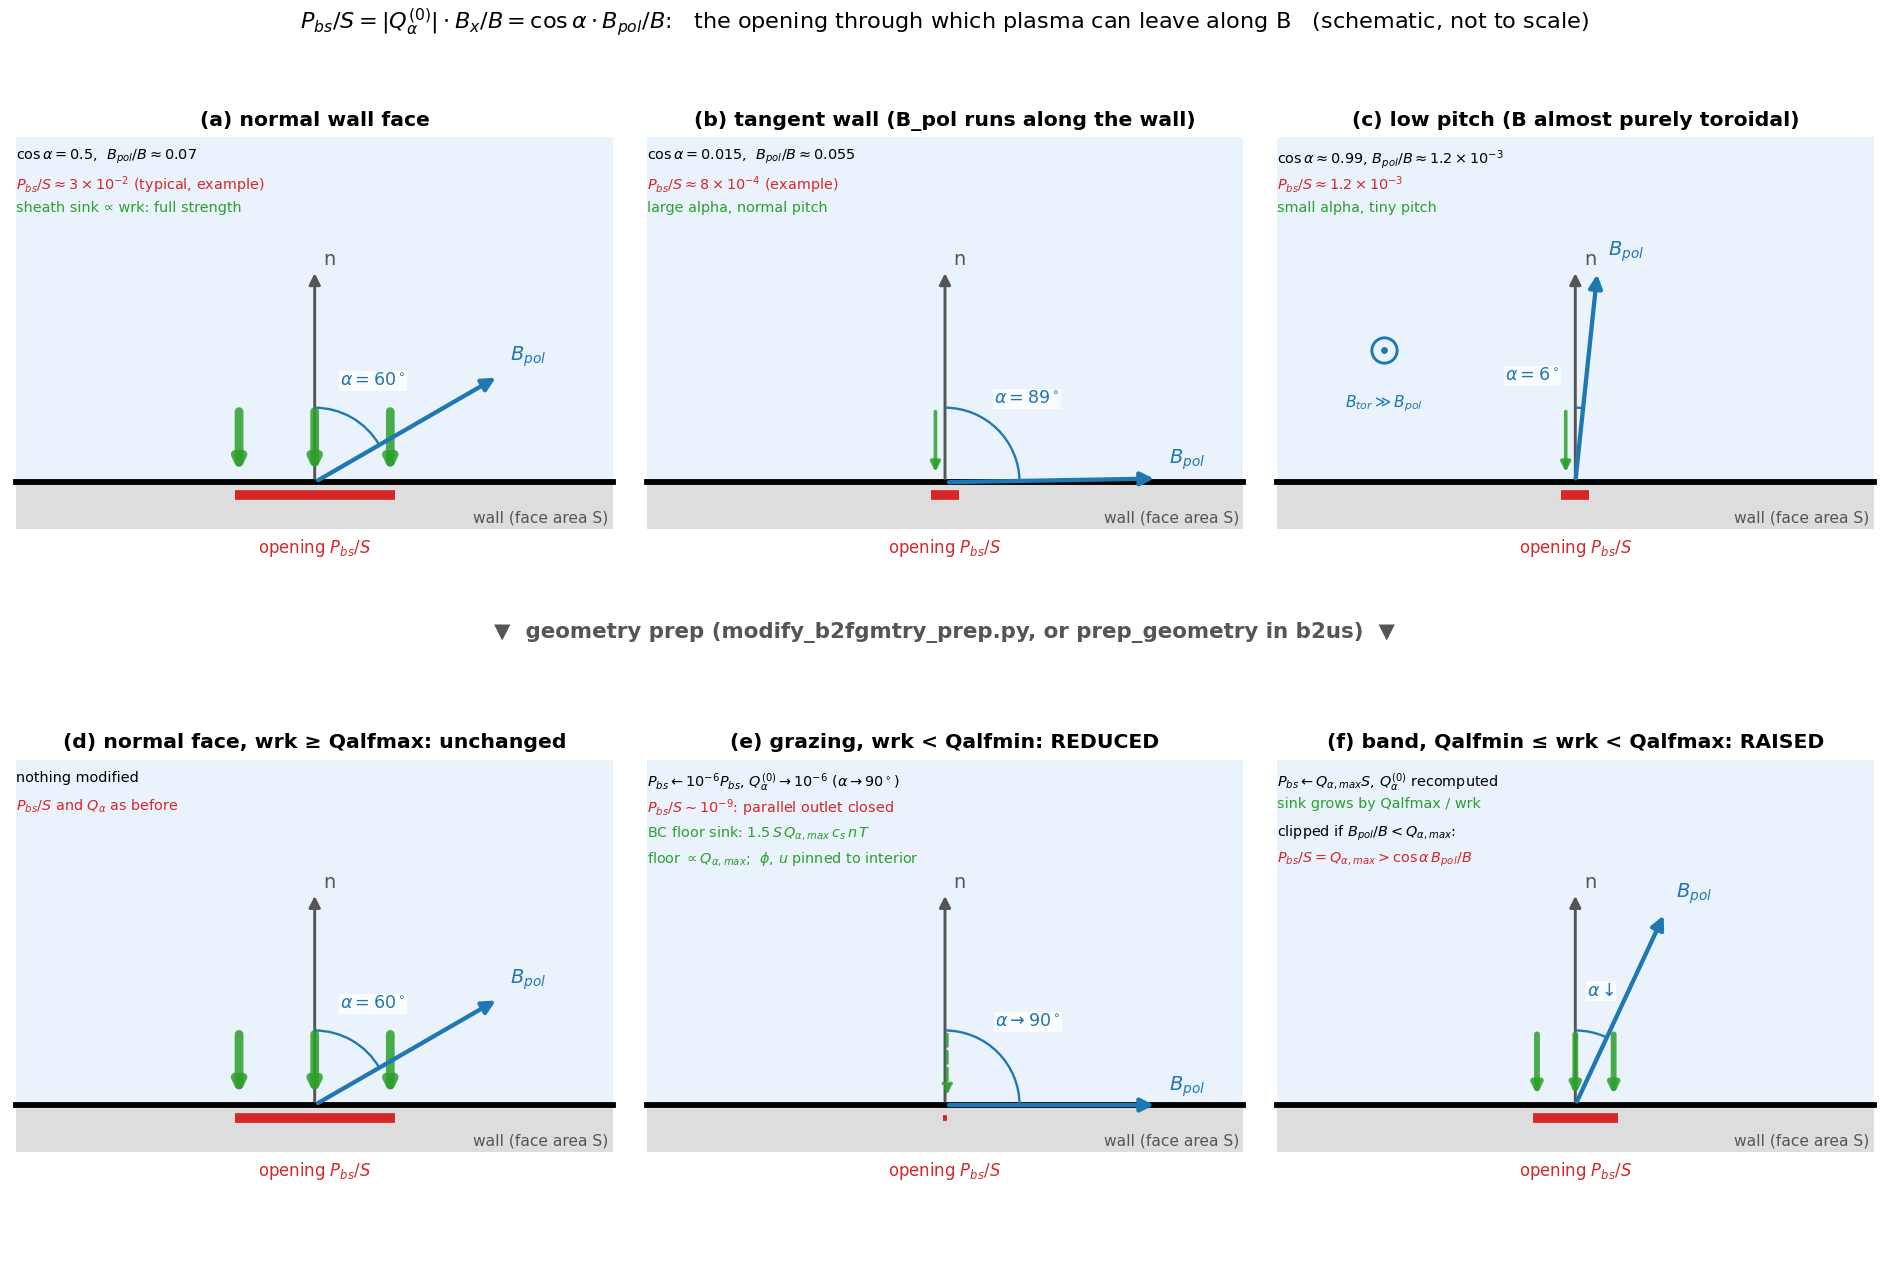
\includegraphics[width=\linewidth]{qalf_sketch.png}
\caption{Schematic (not to scale) of one wall face in the poloidal plane: wall (hatched), face normal $n$, poloidal projection
of $\mathbf{B}$ (blue) at angle $\alpha$ to the normal, opening $P_{bs}/S$ (red bar) and the resulting sink (green).
Top: (a) normal face, (b) tangent wall, (c) low pitch. Bottom: the effect of the prep step on (d) a normal face (unchanged),
(e) a grazing face (reduced), (f) a face in the band $[\qmin,\qmax)$ (raised). Numbers are examples.}
\label{fig:sketch}
\end{figure}

%======================================================================================
\section{Where $P_{bs}$ and $Q_\alpha$ are used in the equations}\label{sec:eqs}
B2.5 evolves the parallel velocity $u_\parallel$; the poloidal projection of a parallel flux through a face is
$P_{bs}\times$(flux density).

\begin{longtable}{p{4.2cm}p{4.0cm}p{6.4cm}}
\toprule
Routine (line) & Expression & Role \\ \midrule
\endhead
\code{b2tfnb.F:423} & \code{flo(:,0)=fcPbs*wrk0+...} & poloidal particle flux $=P_{bs}\,\overline{u_a}\,n$ plus diffusive and drift parts \\
\code{gradc_div_par.F:46} & \code{wrkf=funf*fcPbs} & parallel gradient/divergence of a cell quantity \\
\code{b2sihs_.F:221} & \code{wrkf*fcPbs} & $\nabla\!\cdot(u_e)$ work terms in the energy sources \\
\code{b2news_.F:440} & \code{-fch_p/(qe*(fcPbs+cutlo))} & electron parallel velocity from the parallel current \\
\code{b2tlhe.F}, \code{b2tlhi.F} & \code{chvemx=cflme*sqrt(T/m)*|fcPbs|} & free-streaming flux limit: allowed flux $\propto P_{bs}$ \\
\code{b2tlmv.F:78} & \code{qfl=cflmv*|fcPbs|*...} & parallel viscosity flux limit \\
\code{b2nxfc.F:88} & \code{flub+fcPbshz*wrkf} & momentum/convective coefficients \\
\code{calccoef.F:52--110} & weights \code{Qalf}, \code{Qbet}, \code{Qgam} & conductive flux $=\text{con}_0\,\Delta_{\rm cell}+\text{con}_1\,\Delta_{\rm vertex}$ with $t_{00}=\cos\alpha$, $t_{10}=\sin\alpha$, $t_{01}\propto\sin\beta$, $t_{11}\propto\cos\beta$ \\
\code{b2txcx.F}, \code{b2txcy.F}, \code{b2txcc.F} & \code{Qalf/Qgam**} factors & face conductances contain $\cos\alpha/\cos\gamma$ \\
\code{b2tfhe_.F:134,152} & \code{chce(:,0)*fcQalf(:,0)}, \code{chce(:,1)*fcQalf(:,1)} & conductivity components weighted with $\cos\alpha$, $\sin\alpha$ \\
\code{b2us_feedback.F:1832} & skip face if \code{|Pbs/S|<Qalfmin} & feedback loops ignore grazing faces \\
\code{b2trno.F:377} & \code{wrk0>=Qalfmin} & with \code{b2trno_set_chcb_0=1}: radial coefficients zeroed on wall faces \\
\bottomrule
\end{longtable}

Wherever $P_{bs}$ is tiny, the cell on the other side of that face is magnetically disconnected from its neighbour
(through that face), and every flux limit based on $|P_{bs}|$ is tiny as well.

%======================================================================================
\section{Boundary conditions on wall faces}\label{sec:bc}
\subsection{What is implemented}
The conditions are applied in \code{b2stbc_phys.F} as sources in the equation of the \emph{guard} cell.
Each source is written $S_0+S_1\,X$: index~0 the explicit part, index~1 the coefficient multiplying the guard-cell
unknown $X$ ($n_a$, $u$, $T_e$, $T_i$ or $\phi$). The quantities used below are:
$S$ the face area, $\wrk=|\qalf^{(0)}B_x/B|$ (computed from the \emph{stored angles}, not from $P_{bs}$),
$c_s=\sqrt{p_z/\rho_z}$ (for \code{mompar(.,.,2)}$<0.5$, otherwise $\sqrt{(T_eZ+T_i)/m}$), $m_{par}=$\code{mompar(.,.,1)},
$\gamma_e$ the sheath transmission, and $f=\pm1$ the face orientation (\code{bcFcOr}). The conditions that matter for
a wall segment with \code{bccon}=14, \code{bcmom}=13, \code{bcene}=15, \code{bceni}=15, \code{bcpot}=11 are listed in
Table~\ref{tab:bc}. Every one of them tests the \emph{same} criterion, $\wrk<\qmin$.

\begin{table}[ht]
\centering\small
\renewcommand{\arraystretch}{1.35}
\begin{tabular}{p{2.5cm}p{6.4cm}p{6.0cm}}
\toprule
Condition (line) & Normal face: $\wrk\ge\qmin$ & Grazing face: $\wrk<\qmin$ \\ \midrule
particles, \code{BCCON=14} (1309) &
  $S_1=-S\,m_{par}\,c_s\,\wrk$ \quad(more precisely $-S\,m_{par}\max(c_s|\wrk|,\,v_{bc}\,\mathrm{sgn}\,\wrk+v_{bnd})$) &
  $S_0=0$,\ $S_1=-S\,m_{par}\,c_s\,\qmax$ \\
parallel momentum, \code{BCMOM=13} (3294) &
  $u_{\rm guard}\,|P_{bs}h_z| = m_{par}\,v_{bc}\,S\,h_z$, i.e.\ $u_{\rm guard}=\pm m_{par}c_s\,\dfrac{S\,\wrk}{|P_{bs}|}$; weight $U_{BIG}/\varepsilon^2$ &
  $u_{\rm guard}=u_{\rm interior}-\texttt{cor9}\,(\ldots)$, weight $V_{BIG}=10^{-2}U_{BIG}$ \\
electron energy, \code{BCENE=15} style~1 (4496) &
  $s_1=|P_{bs}|$ &
  $s_1=S\,\qmax$ \\
 & \multicolumn{2}{p{12.6cm}}{common to both: $t_0=s_1\,n_e\sqrt{1/2\pi}\,v_{te}\,\exp\!\bigl(-e(\phi-\phi_{pot})/T_e\bigr)$;\ \
   $S_1=-[(1+\gamma_e+\texttt{enepar1})+\texttt{stab\_te}]\,t_0$;\ \
   $S_0=-[(1-\gamma_e)\,e(\phi-\phi_{pot})-\texttt{stab\_te}\,T_e]\,t_0$;\ \
   zeroed if \code{b2nppo_restr_po}$\ne0$ and $S_0+S_1T_e>0$} \\
ion energy, \code{BCENI=15} style~0 (6061) &
  $S_1=-\texttt{enipar1}\,\sum_s m_{par}\,n_s\,S\,c_s\,\wrk-\texttt{stab\_ti}\,n_e\,c_s\,S$;\ \ $S_0=+\texttt{stab\_ti}\,n_e\,c_s\,S\,T_i$ &
  $S_0=0$,\ $S_1=-1.5\,S\,\qmax\,c_s\,n_i$ (no stabilizer) \\
potential/current, \code{BCPOT=11} (7586) &
  current continuity with $S\wrk$: $I_i=e\sum Z m_{par}S c_s\wrk\,n_s$,\ $I_e=e\,n_e\sqrt{1/2\pi}\,v_{te}\,S\wrk\,\exp(\ldots)$;\
  $S_0=(1-\gamma_e)I_e-I_i+t'\phi$,\ $S_1=-t'$ &
  $\phi_{\rm guard}=\phi_{\rm interior}-\texttt{cor9}\,(\ldots)$, weight $P_{BIG}S$ (no sheath current relation) \\
\bottomrule
\end{tabular}
\caption{Boundary conditions on a wall face, normal versus grazing. The grazing branch always replaces the true contact
fraction $\wrk$ (or $P_{bs}/S$) by the constant $\qmax$ in the sinks, and pins $u$ and $\phi$ to the interior cell.
\texttt{cor9} is \texttt{b2stbc\_BC2\_cor9} (default 0): with the default the pinned values are exactly the interior ones.}
\label{tab:bc}
\end{table}

\paragraph{Notes.}
\begin{itemize}
\item Drift terms ($v_{bnd}$ with \code{vaecrb}, \code{vadia}, and the \code{*PSch} Pfirsch--Schl\"uter terms) are zero in
      a run without drifts.
\item With \code{bceni_15_style=1} the ion-energy sink is instead $\propto(1+\texttt{stab\_ti})\,t_0\,c_s\,|P_{bs}|$ (line 6123) and
      there is \emph{no} grazing branch: the $\qmin$ test only exists for \code{bceni_15_style=0}.
\item If \code{conpar(.,.,2)}$>0$, an extra anomalous-diffusion sink $\propto\mathrm{d}na_0\,S/\texttt{conpar2}$ is added (not discussed here).
\item The sheath stabilization coefficients add an implicit diagonal $+\mathrm{stab}\times(\text{flux factor})$ and the
      matching explicit part $+\mathrm{stab}\times T_{\rm old}\times(\text{same factor})$, so the net source at the current
      iterate is unchanged. For the ions with style~0 the factor is $n_e c_s S$, \emph{not} $P_{bs}$.
\end{itemize}

\subsection{Behaviour in the different regimes}\label{sec:regimes}
Let $\wrk$ denote the angle-based value of the stored file, and $P_{bs}/S$ the stored contact fraction. The cases
(a)--(f) refer to Figure~\ref{fig:sketch}.

\begin{longtable}{p{3.4cm}p{3.6cm}p{7.6cm}}
\toprule
Case & State in the file & What the conditions of Table~\ref{tab:bc} see \\ \midrule
\endhead
(a), (d) normal, $\wrk\ge\qmax$ & $P_{bs}=S\wrk$; unchanged by the prep &
   normal branch, all rows consistent; momentum gives $u_{\rm guard}=\pm m_{par}c_s$ \\
(b), (c) before the prep, $\wrk<\qmin$ & original $P_{bs}=S\wrk$ &
   grazing branch with the \emph{stored} $\qmax$ (default $10^{-3}$): floor $\qmax S$; $u$, $\phi$ pinned; the bulk face fluxes
   $\propto P_{bs}$ and $\qalf^{(0)}$ are small but not zero \\
(c) low pitch with $\qmin\le\wrk<\qmax$ & $P_{bs}=S\wrk$ &
   normal branch with the small $\wrk$ (sinks $\propto\wrk$); becomes grazing if $\qmin$ is raised above $\wrk$ \\
(e) reduced, $\wrk<\qmin$ & $P_{bs},\,\qalf^{(0)}\to f_{\rm red}\times$ original ($\alpha\to90^\circ$) &
   grazing branch with floor $\qmax S$ (the \emph{new} $\qmax$ if it was changed); bulk face fluxes
   $\propto P_{bs},\qalf^{(0)}$ essentially zero: the parallel outlet is closed \\
(f) raised, $\qmin\le\wrk<\qmax$, unclipped & $P_{bs}=\qmax S$, $\qalf^{(0)}$ recomputed, $\wrk=\qmax$ &
   normal branch with $\wrk=\qmax$; all rows consistent; $u_{\rm guard}=\pm m_{par}c_s$; sink larger by $\qmax/\wrk_{\rm old}$ \\
(f) raised, clipped, $B_x/B<\qmax$ & $P_{bs}=\qmax S$ but $\qalf^{(0)}$ clipped to $\pm1$, so $\wrk=B_x/B$ &
   see Section~\ref{sec:clip}: rows using $\wrk$ see $B_x/B$, rows using $P_{bs}$ see $\qmax$ \\
\bottomrule
\end{longtable}

\paragraph{Continuity of the sink at $\qmin$.} With the prep applied, a face just above $\qmin$ is raised to
$\wrk=\qmax$, and a face just below gets the floor $\qmax S$: both give $\propto\qmax S$. If only the scalars are edited in the file
without the prep, a face just above $\qmin$ keeps its true $\wrk\approx\qmin$ while a face just below gets $\qmax S$, so the
sink jumps by $\qmax/\qmin$.

\subsection{Clipped faces}\label{sec:clip}
A face cannot have $P_{bs}/S$ larger than $B_x/B$ (the case $\qalf^{(0)}=1$). When the prep (or the Python port) raises a face to
$P_{bs}/S=\qmax$ and $B_x/B<\qmax$, $\qalf^{(0)}$ is clipped to~1, so afterwards
\[
   \frac{P_{bs}}{S}=\qmax\ \ >\ \ \left|\qalf^{(0)}\frac{B_x}{B}\right| = \frac{B_x}{B}.
\]
The Fortran prep does exactly the same. The boundary conditions of Table~\ref{tab:bc} then see different values
depending on which quantity they use:
\begin{center}\small
\begin{tabular}{lll}
\toprule
Condition & uses & sees \\ \midrule
particles, ion energy (style~0), potential & $\wrk=|\qalf^{(0)}B_x/B|$ & $B_x/B$ (no increase) \\
electron energy & $|P_{bs}|$ & $\qmax$ (increased) \\
parallel momentum & both: $u_{\rm guard}=\pm m_{par}c_s\,S\wrk/|P_{bs}|$ & $\pm m_{par}c_s\,(B_x/B)/\qmax$ \\
\bottomrule
\end{tabular}
\end{center}
The momentum condition therefore forces a guard-cell velocity of only $(B_x/B)/\qmax$ times the sound speed: \emph{subsonic}
(the Bohm criterion is not imposed) on clipped faces. The stored $P_{bs}$ is also used by the bulk fluxes and flux limits.
A way to keep a file self-consistent is to cap $P_{bs}$ at $S\,B_x/B$ on such faces (not implemented in the Fortran).

%======================================================================================
\section{The geometry prep step (\texttt{b2us\_prep})}\label{sec:prep}
\subsection{Parameters}
\begin{longtable}{p{4.6cm}p{2.0cm}p{8.0cm}}
\toprule
Parameter (\code{b2us_prep_...}) & Default & Meaning \\ \midrule
\endhead
\code{Qalfmin} & $10^{-3}$ & wall-face threshold in $\wrk$; stored in \code{b2fgmtry} \\
\code{Qalfmax} & $10^{-3}$ & minimum contact fraction assigned to wall faces / floor sink in the BCs; stored in \code{b2fgmtry} \\
\code{Pbs_reduce_fac} & $10^{-3}$ & factor applied to $P_{bs}$ of faces with $\wrk<\qmin$ \\
\code{mod_hc} & 0 & recompute \code{fcHc} on boundary faces (effective cells); recommended with \code{b2txcx_increase_transp_coefs}$>1$ \\
\code{set_beta_0} & 0 & set $\beta=0$ on faces between boundary cells of the same tube; same recommendation \\
\code{Qalf_mod_style} & 0 & 0: wall $\iff\wrk\ge\qmin$; 1: end-of-tube faces and neighbours \\
\bottomrule
\end{longtable}

\subsection{Algorithm for \texttt{Qalf\_mod\_style}$=0$}
(\code{b2us_prep.F}, lines 2595--2735.) For every guard face with \code{fcLbl}$>0$, with $b_z=\pm1$ the sign of \code{cvEb(guard,2)}:
\begin{enumerate}
\item $\wrk=|\qalf^{(0)}B_x/B|$; the face is a \emph{wall face} iff $\wrk\ge\qmin$.
\item \textbf{Wall face with $\wrk<\qmax$:}
      \begin{align*}
      P_{bs}&\leftarrow \qmax\,S\,\mathrm{sign}(P_{bs}),\\
      \qalf^{(0)}&\leftarrow \mathrm{clip}\!\left(\frac{P_{bs}}{S}\frac{B}{B_x},-1,1\right),\quad
      \qalf^{(1)}\leftarrow \mathrm{sign}(\qalf^{(1)})\sqrt{1-(\qalf^{(0)})^2}.
      \end{align*}
\item \textbf{Every wall face:} $\qbet^{(0)}=\pm b_z$ (sign of $\qalf^{(0)}$), $\qbet^{(1)}=0$, $\qgam^{(0)}=|\qalf^{(0)}|$,
      $\qgam^{(1)}=\pm\qalf^{(1)}b_z$. That is, $\beta=0$ and $\gamma=\alpha$: the connector from interior to guard cell
      is declared parallel to $\mathbf{B}$.
\item \textbf{Grazing face ($\wrk<\qmin$):} $P_{bs}\leftarrow f_{\rm red}P_{bs}$, $\qalf$ recomputed from the new $P_{bs}$ as in step~2,
      and $\qbet$ recomputed from the unchanged $\qgam$ with the relation of Section~\ref{sec:defs}.
\end{enumerate}
Optionally \code{mod_hc} rescales \code{fcHc} on the boundary faces and \code{set_beta_0} sets $\beta=0$ on tube faces
next to the boundary.

\paragraph{Meaning of step 3.} In \code{calccoef} the flux through a face is
$\text{con}_0\,\Delta_{\rm cell}+\text{con}_1\,\Delta_{\rm vertex}$ with weights $\cos\alpha$, $\sin\alpha$ on the cell
difference and $\propto\sin\beta$, $\cos\beta$ on the tangential vertex difference. With $\beta=0$ the large parallel
conductivity no longer couples to the tangential difference, and the factor $\cos\alpha/\cos\gamma$ in the
conductances is 1. For faces whose guard cell was already built with the connector along $\mathbf{B}$ ($\beta\approx0$)
this changes nothing; for faces with a connector at a large angle to $\mathbf{B}$ it changes the conduction through the face
substantially, in a direction that depends on the geometry. This part of the prep is a separate physics choice from the
$Q_{\alpha}$/$P_{bs}$ treatment.

\subsection{Who calls the prep, and the unstructured path}
\code{prep_geometry} is called from \code{preprocessing/b2agdr_st.F:625} (structured grid converted inside
\code{b2ag}) and \code{convert/b2us.F:186}. The unstructured driver \code{b2agdr.F} (traduit input,
\code{*format unstructured} in \code{b2ag.dat}) calls only \code{b2agfs}, \code{b2agmt} and, if
\code{b2agdr_redef_gmtry}$\ne0$, \code{b2agbs}; it \emph{never} calls the prep. Hence in \code{b2ag.log}:
\begin{lstlisting}
*** IPMAIN--WARNING: parameter has been set but not read: b2us_prep_qalfmin
*** IPMAIN--WARNING: parameter has been set but not read: b2us_prep_qalfmax
... (mod_hc, pbs_reduce_fac, set_beta_0 likewise)
\end{lstlisting}
At run time \code{b2us_geo.F:345--354} reads \code{Qalfmin}/\code{Qalfmax} from \code{b2fgmtry} \emph{after} the input
parameter, so the value in the file wins. A file produced by the unstructured \code{b2ag} therefore carries the defaults
$10^{-3}/10^{-3}$ regardless of \code{b2ag.dat}. Note also that \code{b2agdr_redef_gmtry '0'} disables the
flux-constancy correction \code{b2agbs}, which is on by default since 3.0.6.

%======================================================================================
\section{What reducing the values means physically}\label{sec:phys}
\begin{itemize}
\item \textbf{$P_{bs}\to0$ on a face} means: no field line crosses it in the poloidal projection, or, in B2.5's 2D
      picture, the flux tube does not end on that piece of wall. Parallel convection, parallel conduction and the sheath
      sink through that face vanish in the bulk equations.
\item \textbf{Reducing by $f_{\rm red}$} is the numerical way of saying ``this is not a target''. The face keeps a nonzero value
      only to avoid divisions by zero (\code{fcPbs+cutlo}).
\item \textbf{$\qmax$ as a floor} (grazing faces): a regularised, small, non-physical sink $\propto S\,\qmax\,c_s\,n$ representing,
      loosely, ``some plasma still reaches the wall'' (cross-field transport, field-line tilt below the resolution of the 2D grid).
      Its size is a modelling choice.
\item \textbf{$\qmin$} is where the code stops trusting the stored angle: below it the wall is not a sheath; above it,
      the sheath applies with the true projection.
\item \textbf{Insulating potential:} on grazing faces the guard potential is pinned to its interior neighbour, so
      the sheath current relation is not applied there.
\end{itemize}

For a flux tube that ends on a face with tiny $\wrk$, the end cell has (i) an almost closed parallel outlet, (ii) a flux
limit $\propto|P_{bs}|$ that is tiny, and (iii) at most the fixed floor sink. Plasma arriving along the tube must leave
radially or accumulate in the end cell (``dead end''); this is the situation to look for when density, temperature or
parallel velocity pile up at the end of a flux tube that touches the wall at a shallow angle.

%======================================================================================
\section{Practical consequences}\label{sec:practice}
\begin{itemize}
\item \textbf{Where the effect is largest.} The sinks of the normal branch scale with $\wrk$, so the strongest effect is on the
      faces with the smallest $\wrk$; the floor $\qmax S$ is the only sink left on grazing faces. Raising $\qmax$ strengthens
      the floor on every grazing face in proportion, and strengthens the raised faces by $\qmax/\wrk_{\rm old}$ (at most
      $\qmax/\qmin$).
\item \textbf{Energy balance of an end cell.} Whether heat still accumulates at a grazing contact is a balance between the
      new sink and whatever source or flux feeds the end cell. A useful check is the net ion/electron heat leaving the end cell
      through each of its faces (from the face fluxes in the plasmastate), before and after the change.
\item \textbf{Potential and current.} Grazing faces have no sheath current relation; if current has no other sink the potential in
      adjacent cells can drift. Faces just above $\qmin$ have a sheath current capacity $\propto\wrk$, i.e.\ very small.
\item \textbf{The potential cap.} The ratio limiter \code{b2nppo_restr_po} limits $|e\phi|\le\texttt{restr\_po}\times T_e$ locally. In cold cells
      (low $T_e$ or at the temperature floor) the cap is much smaller than the potential imposed by the neighbours, so a tight cap
      can conflict with charge conservation. This interacts with any change of the wall treatment and should be
      varied separately.
\item \textbf{Change one thing at a time.} Geometry (Qalf/Pbs), angle overwrite ($\beta=0$), floors/caps and the start state
      each change the wall problem; compare short start-up runs from the same state in separate run directories.
\end{itemize}

%======================================================================================
\section{Tools}\label{sec:tools}
\begin{longtable}{p{4.8cm}p{9.8cm}}
\toprule
Script & Purpose \\ \midrule
\endhead
\code{modify_b2fgmtry_prep.py} & Python port of the wall-face part of the prep for unstructured \code{b2fgmtry}: \code{--qmin --qmax --pbs-reduce}.
   Checks a byte-exact read/write round trip first, never overwrites the input unless \code{--inplace} (original kept as \code{.orig}),
   refuses \code{-o} equal to the input. \code{--angles keep} (default) leaves $\qgam$ alone and recomputes $\qbet$ only on raised faces;
   \code{--angles prep} also overwrites $\qbet,\qgam$ on all wall faces. \code{--scalars-only} stores just \code{Qalfmin}/\code{Qalfmax}.
   \code{--dry-run} prints the summary only. Not ported: \code{mod_hc}, \code{set_beta_0}, \code{Qalf_mod_style=1}. \\
\code{plot_qalf_wall.py} & Maps the wall faces. Default: classes by $\wrk$ (core-type, grazing, band, normal).
   \code{--ref ORIG}: classes from the original file, coloured by whether the prepared file was actually reduced/raised.
   \code{--show pbs}: stored $\log_{10}(|P_{bs}|/S)$. \code{--show dpbs} (with \code{--ref}): $\log_{10}$ of the ratio to the original.
   \code{--compare Q2} circles faces whose grazing status differs for another $\qmin$; \code{--list N} prints the faces. \\
\code{sketch_qalf_pbs.py} & Regenerates the schematic of Figure~\ref{fig:sketch}. \\
\bottomrule
\end{longtable}

\paragraph{Reading the plots.} Without \code{--ref} the plot shows the file as the code will see it (the classification of the
boundary conditions uses the angle-based $\wrk$). With \code{--ref} the plot shows what was done to the file compared with the
original; the two differ on raised faces, which move to $\wrk=\qmax$, and on clipped faces, whose angle-based $\wrk$ stays below $\qmax$.

%======================================================================================
\section{Recommendations}
\begin{enumerate}
\item Always keep the unmodified \code{b2fgmtry} and generate variants from it into new file names; the prep is not idempotent
      (reducing twice multiplies $P_{bs}$ by $f_{\rm red}^2$).
\item Keep $\qmax\ge\qmin$ and, if editing only the scalars, prefer equal values to avoid the jump in the sink at $\qmin$.
\item Decide explicitly whether to overwrite the connector angles ($\beta=0$, $\gamma=\alpha$); on a grid built with the connector along
      $\mathbf{B}$ the overwrite changes little, otherwise it is a separate physics choice.
\item Inspect clipped faces ($B_x/B<\qmax$): either accept the inconsistency or cap $P_{bs}$ at $S\,B_x/B$.
\item Remove or comment the unused \code{b2us_prep_*} lines in \code{b2ag.dat} on the unstructured path so the log does not suggest
      they are active.
\item If a parameter set comes from a case built through the structured $\to$ \code{b2us} route, ask how the geometry was produced: the prep step
      only exists there.
\end{enumerate}

%======================================================================================
\section*{Appendix: source locations}
\begin{longtable}{p{5.0cm}p{9.6cm}}
\toprule
File & Content \\ \midrule
\code{modules/b2us_geo.F:226-227} & defaults $\qmin=\qmax=10^{-3}$ \\
\code{modules/b2us_geo.F:345-354, 404-407} & read (file overrides input) and write of the scalars \\
\code{modules/b2us_geo.F:954} & \code{fcPbshz = fcPbs*fcHz} at file read \\
\code{modules/b2us_prep.F:2494-2503} & reads of the \code{b2us_prep_*} parameters \\
\code{modules/b2us_prep.F:2595-2735} & wall-face classification, raising, reduction, \code{mod_hc} per face \\
\code{modules/b2us_prep.F:2741-2803} & boundary ordering, \code{cvAlongBoundary}, \code{set_beta_0} \\
\code{modules/b2us_prep.F:2909ff} & \code{mod_hc} effective-cell recalculation \\
\code{sources/b2stbc_phys.F:605-643} & \code{csbc_is}, \code{vbc_is}: $c_s$, $\wrk$, $v_{bnd}$, $v_{bc}$ \\
\code{sources/b2stbc_phys.F} 1309, 3294, 4496, 6061, 6123, 7586 & BC branches (Table~\ref{tab:bc}) \\
\code{sources/b2stbc_phys.F:238-248} & $\varepsilon$, $U_{BIG}$, $V_{BIG}$, $P_{BIG}$, \code{cor9} \\
\code{utility/calccoef.F:52-110} & use of $\qalf,\qbet$ in the face flux \\
\code{transport/b2trno.F:377} & \code{set_chcb_0} use of $\qmin$ \\
\code{modules/b2us_feedback.F:1832} & feedback skips grazing faces \\
\code{preprocessing/b2agdr.F}, \code{b2agdr_st.F:625}, \code{convert/b2us.F:186} & who calls the prep \\
\bottomrule
\end{longtable}

\end{document}
